\chapter[Player/Stage/Gazebo ]{Player/Stage/Gazebo \label{chap:gazebo}}
\chaptermark{Player/Stage/Gazebo}
	Symulator \mbox{\texttt{Player/Stage/Gazebo}} został już opisany w pracy inżynierskiej \cite{inzynierka} jednak z uwagi na jego ważną rolę i zmiany jakie zdecydowano się wprowadzić w symulowanym
	środowisku podczas rozwijania aplikacji zdecydowano się na krótkie przypomnienie koncepcji projektu.

	\section{Koncepcja}
	Oprogramowanie składa się z trzech niezależnych aplikacji \textit{Player}, \textit{Stage} oraz \textit{Gazebo}.
	\textit{Gazebo} oraz \textit{Stage} są środowiskami symulacyjnymi. Z tą różnicą, że \textit{Stage} jest środowiskiem dwuwymiarowym, dedykowanym do symulowania dużych populacji robotów
	mobilnych. Natomiast \textit{Gazebo} zapewnia pełną trójwymiarową symulację, uwzględniając również oddziaływania fizyczne pomiędzy stosowanymi obiektami.
	W trakcie realizacji niniejszej pracy wydana została pierwsza stabilna wersja oprogramowania dostępna pod adresem \url{http://gazebosim.org}.
	Wcześniej wszelkie dane dotyczące wszystkich aplikacji wchodzących w skład projektu dostępne były na stronie \url{http://playerstage.sourceforge.net}. Z uwagi na trudności związane z adaptacją
	symulatora zdecydowano się na kontynuację prac na wersji pobranej ze starego repozytorium.
	Ostatnia aplikacja wchodząca w skład projektu, czyli \textit{Player} jest serwerem sieciowym służącym do sterowania rzeczywistymi robotami. Dostarcza prosty interfejs, wspierający komunikację z wieloma 
	typami powszechnie stosowanych czujników i aktuatorów.
	Oprogramowanie jest kompatybilne z systemami Linux, Solaris, *BSD oraz Mac OSX.
	W niniejszej pracy zdecydowano się na wykorzystanie jedynie symulatora \textit{Gazebo}.

	\section{Architektura symulatora}
	\begin{figure}[!b]
	\centering
	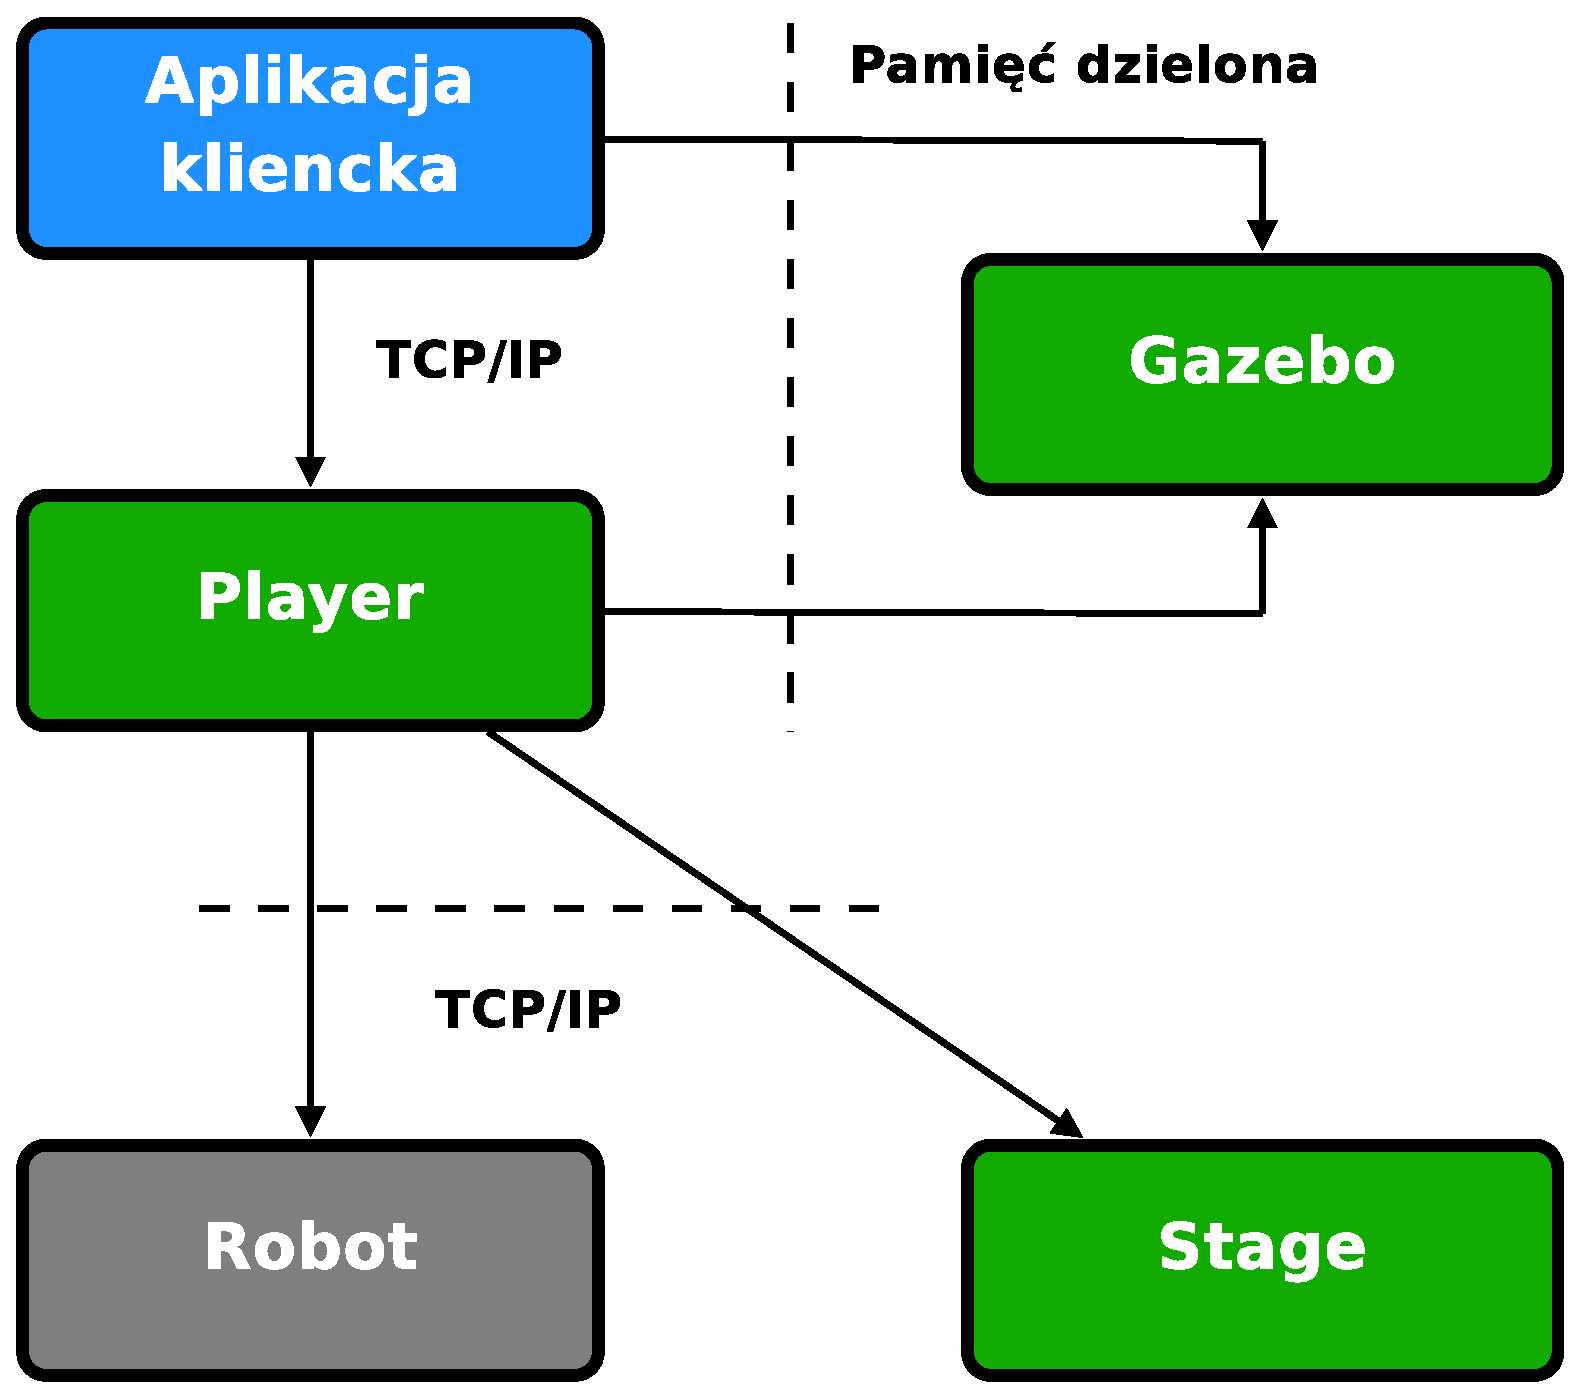
\includegraphics[scale=0.3]{./gazebo/architektura}
	\caption{Schemat komunikacji w środowisku \textit{Player/Stage/Gazebo} \label{fig:arch}}
	\end{figure}
	
	Wymiana informacji pomiędzy elementami środowiska symulacyjnego \textit{Player/Stage/Gazebo} została przedstawiona na 
	rysunku~\ref{fig:arch}.
	Po zapoznaniu się z nim , można lepiej zrozumieć rolę programu \textit{Player}. Pełni on funkcję pośrednika pomiędzy aplikacją klienta, stworzoną przez użytkownika
	a rzeczywistym robotem lub symulatorami modelującymi jego zachowanie w tym przypadku (\textit{Stage} lub \textit{Gazebo}). 
	Komunikacja pomiędzy \textit{Player-em}, robotem oraz aplikacją kliencką realizowana jest za pomocą protokołu TCP/IP.
	Dzięki takiej architekturze z punktu widzenia klienta nie istotne jest, czy interfejsy udostępnione przez \textit{Player-a} sterują rzeczywistym robotem, czy symulowanym odpowiednikiem.
	
	Z samym symulatorem, zarówno \textit{Stage} jak i \textit{Gazebo} można komunikować się poprzez pamięć współdzieloną (rysunek \ref{fig:wybrana_arch}), bez wykorzystywania aplikacji \textit{Player}. Rozwiązanie to jest 
	preferowane w sytuacji gdy korzystanie z \textit{Playera} nie jest uzasadnione, lub kiedy użytkownik dokonał modyfikacji działania symulatora, których nie implementuje \textit{Player}. 
	Aplikacja \textit{Gazebo} udostępnia w tym celu  bibliotekę \textit{libgazebo}, dostarczającą zestaw funkcji do komunikacji.
	\begin{figure}[h]
	\centering
	\includegraphics[scale=0.3]{./gazebo/wybrana_architektura}
	\caption{Zrealizowany schemat komunikacji w środowisku \textit{Player/Stage/Gazebo} \label{fig:wybrana_arch}}
	\end{figure}
	Z tego właśnie rozwiązania zdecydowano się skorzystać w niniejszej pracy. Po pierwsze, dlatego iż zmniejsza to nakład niezbędnych prac, po drugie iż nie posiadano rzeczywistego modelu
	zawodnika. Wprowadzone poprawki podczas opracowania środowiska testowego oraz przygotowanie własnego sterownika robota, także nasunęły to rozwiązanie.

	Podsumowując, struktura pakietu oprogramowania \mbox{\textit{Player/Stage/Gazebo}} umożliwia tworzenie aplikacji sterujących robotami w sposób,
	który zapewnia przenośność stworzonych programów i ich działanie zarówno na symulatorach robotów, jaki i na rzeczywistych obiektach.
	
 	\subsection{Gazebo}
 	
 	Symulator \textit{Gazebo} jak wynika z wcześniejszego tekstu, umożliwia symulację grup robotów mobilnych. Symulowane
 	środowisko jest w pełni trójwymiarowe, uwzględniona jest dynamika brył oraz obliczane rzeczywiste oddziaływania między komponentami symulowanego świata.
	Okupione jest to oczywiście większym niż w przypadku \textit{Stage} zużyciem mocy obliczeniowej, dlatego symulowane populacje robotów nie powinny być zbyt liczne.
 	 	
 	Trzy najistotniejsze komponenty wykorzystywane przez program \textit{Gazebo} to:
 	\begin{itemize}
 	 \item ODE\footnote{Open Dynamics Engine, \url{http://www.ode.org}}, biblioteka  odpowiadająca za symulację
 	 	zależności fizycznych pomiędzy bryłami oraz detekcję kolizji,
 	 \item OGRE\footnote{Object-Oriented Graphics Rendering Engine, \url{http://www.ogre3d.org/}}, 
		silnik graficzny umożliwiający tworzenie wspomaganej sprzętowo grafiki 3D,
 	 \item FLTK\footnote{Fast Light Toolkit, \url{http://www.fltk.org/}}, biblioteka dostarczająca 
		przenośny interfejs użytkownika dla \textit{Gazebo}.
 	\end{itemize}

	W \textit{Gazebo} możliwe jest symulowanie standardowych sensorów stosowanych w robotyce (m.in. czujniki odległości, kamery, GPS). Symulator wyposażony jest w gotowe modele 
	popularnych robotów (jak np. \textit{Pioneer2DX}, \textit{Pioneer 2AT} oraz \textit{SegwayRMP}).
	Dozwolone jest także tworzenie własnych modeli.
	Środowisko pozwala ponadto na tworzenie własnych modeli brył, z możliwością konfigurowania ich właściwości fizycznych (takich jak np. masa, współczynnik tarcia, sztywność).
	Dzięki temu symulator może w dużym stopniu odzwierciedlać rzeczywistość. Modele można wyposażyć w jeden ze zdefiniowanych kontrolerów umożliwiających sterowanie (zadawanie prędkości, 
	czy odczyt danych z sensorów) lub opracować własny.
	\begin{figure}[!t]
	\centering
	\label{fig:gazebo}
	\includegraphics[scale=0.42]{./gazebo/gazebo_screen}
	\caption{\textit{Gazebo} -- okno główne (wersja 0.10)}
	\end{figure}

	\section{Modelowanie obiektów w Gazebo}
	Tworzenie symulowanego środowiska w \textit{Gazebo} polega na opracowaniu opisu świata w pliku z rozszerzeniem \textit{.world} za pomocą języka XML. W pliku powinny zostać zamieszczone parametry
	określające przebieg symulacji oraz informacje o występujących w danym świecie modelach.
	
	\subsection{Zasady modelowania w Gazebo 0.10}
	Forma pliku \textit{.world} zawierającego opis symulowanego środowiska daje użytkownikowi możliwość konfiguracji wielu kluczowych elementów takich jak: konfiguracja graficznego interfejsu użytkownika,
	zmianę sposobu renderowania sceny, wybór metody detekcji kolizji, zmianę wartości globalnych parametrów symulacji (m.in krok pracy symulatora). Elementy przykładowego pliku \textit{.world} zostały zaprezentowane na listingach poniżej.
	%\small
	%\lstset{language=XML,  basicstyle=\ttfamily\footnotesize,
	\lstset{language=XML,  basicstyle=\ttfamily\scriptsize, 
	commentstyle={}, xleftmargin=20pt, numbers=left, numberstyle=\footnotesize,
	caption={},
	backgroundcolor=\color{light-gray},
	frame=single,
	breaklines=true}
	\begin{lstlisting}[name=gazebo_simple_world]
	<?xml version="1.0"?>
	<gazebo:world>
	\end{lstlisting}
	Bardzo istotnym elementem jest konfiguracja fizyki (ODE), interfejs umożliwia konfigurację globalnych parametrów takich jak:
	\begin{lstlisting}[name=gazebo_simple_world]
	<physics:ode>
		<stepTime>0.001</stepTime>
		<gravity>0 0 -9.8</gravity>		
		<erp>0.8</erp>
		<cfm>0.05</cfm>
		<stepType>quick</stepType>
		<stepIters>25</stepIters>
		<stepW>1.4</stepW>
		<contactSurfaceLayer>0.007</contactSurfaceLayer>
		<contactMaxCorrectingVel>100</contactMaxCorrectingVel>
	 </physics:ode>
	\end{lstlisting}
	\lstset{language=XML,  basicstyle=\ttfamily\footnotesize, 
	commentstyle={}, xleftmargin=20pt, numbers=left, numberstyle=\footnotesize,
	caption={},
	backgroundcolor=\color{light-gray},
	frame=single,
	breaklines=true}
	Znaczenie poszczególnych parametrów jest następujące:
	\begin {enumerate}
	 \item \texttt{stepTime} jest wyrażony w sekundach i określa czas pomiędzy kolejnymi aktualizacjami silnika \texttt{ODE},
	 \item \texttt{gravity} jest wektorem określającym siłę grawitacji,
	 \item \texttt{erp} rozwija się na \textit{error reduction parameter}, przyjmuje on wartości z przedziału od $0$ do $1$ i jest odpowiedzialny za redukcję błędów w połączeniach pomiędzy bryłami
	  (problematyka zostanie szerzej poruszona na stronie \pageref{fig:joints}); \texttt{erp} ustawione na $0$ powoduje, że żadna dodatkowa siła nie jest przykładana do danej bryły, natomiast wartość $1$
	 powoduje, że wszytskie błędy połączeń zostaną naprawione w kolejnym kroku symulatora,
	 \item \texttt{cfm} jest skrótem od \textit{constraint force mixing} i odpowiada za sztywność ograniczeń występujących w kolizjach między bryłami, gdy wartość jest równa $0$ ograniczenie wynikające z fizyki
nie może zostać złamane, ustawienie parametru na wartość dodatnią powoduje, że ograniczenie staje się ``miękkie'', sprężyste,
	  
	 \item \texttt{stepType} odpowiada za rodzaj używanej funkcji z \texttt{ODE} do detekcji kolizji, użytkownik może dokonać wyboru jednej z dwóch wartości:
	      \begin{itemize}
	       \item \textit{world}, używana jest wtedy funkcja \texttt{dWorldStep}, operująca na macierzy zawierającej wszystkie ograniczenia, złożoność obliczeniowa tej metody wynosi $m^3$, natomiast pamięciowa
jest rzędu $m^2$, gdzie $m$ określa ilość wierszy (ograniczeń) analizowanej macierzy,
	       \item \textit{quick}, do detekcji kolizji stosowana jest metoda iteracyjna, w literaturze nazywana \texttt{SOR - Successive over-relaxation} należąca do rodziny metod Gaussa–Seidela, jej złożoność obliczeniowa jest rzędu $m*N$,
		a pamięciowa $m$, gdzie $m$ ma znaczenie jak wyżej,
		natomiast $N$ jest liczbą iteracji; dla dużych systemów metoda jest dużo bardziej wydajna jednak mniej dokładna, mogą także występować problemy z jej stabilnością; najprostszą metodą na poprawę stabilności
		jest zwiększanie \texttt{cfm}, 
	      \end{itemize}
	 \item \texttt{stepIters} - ilość iteracji, gdy do detekcji kolizji wybrano metodę \textit{quick},
	 \item \texttt{stepW} określa czas relaksacji metody Gaussa–Seidela, 
	 \item \texttt{contactSurfaceLayer} określa głębokość na jaką może wnikać bryła w podłoże, ustawienie parametru na małą wartość dodatnią zapobiega jitterowi w momencie, gdy ograniczenia są nieustannie tworzone
	  i zrywane (na przykład podczas ruchu koła po podłożu),
	 \item \texttt{contactMaxCorrectingVel} jest maksymalną korektą prędkości jaka może wynikać z utworzonych tymczasowo kontaktów; domyślnie parametr przyjmuje nieskończoną wartość zmniejszanie jego
	   wartości może zapobiec tworzeniu się zagnieżdżonych kontaktów. 
	\end {enumerate}
	Warto wspomnieć, że niektóre parametry można zmieniać dla poszczególnych modeli lub połączeń \textit{joints}.\newline
	Ustawienia interfejsu: typ (dostępne tylko \textit{fltk}), rozmiaru okna i jego pozycja początkowej:
\begin{lstlisting} [name=gazebo_simple_world]
    <rendering:gui>
        <type>fltk</type>
        <size>640 480</size>
        <pos>0 0</pos>
    </rendering:gui>
\end{lstlisting}
	Określenie parametrów renderowanej sceny: techniki cieniowania, tekstury pokrywającej niebo (dostępne inne opcje, jak np. rodzaje oświetlenia, dodawanie mgły itp.):
\begin{lstlisting} [name=gazebo_simple_world]
    <rendering:ogre>
        <shadowTechnique>stencilAdditive</shadowTechnique>
        <sky>
              <material>Gazebo/CloudySky</material>
        </sky>
    </rendering:ogre>
</gazebo:world>
\end{lstlisting}

	Do tak stworzonego pliku z opisem świata należy następnie dodać modele.  Dodany obiekt musi zawierać co najmniej jeden element \textit{body}, który jest złożony z elementów \textit{geoms}. Sekcja opisująca przykładowy model piłki mogłaby wyglądać następująco:
	\begin{figure}[H]
	\centering
	\includegraphics[scale=0.35]{./gazebo/geoms}
	\caption[Dostępne typy \textit{geoms}]
		{\label{fig:geoms}Dostępne typy \textit{geoms} -- Gazebo 0.10 (źródło:~\cite{gazebo_experts})}
	\end{figure}
	
	\lstset{language=XML,  basicstyle=\ttfamily\footnotesize, 
	commentstyle={}, xleftmargin=20pt, numbers=left, numberstyle=\footnotesize,
	caption={},
	backgroundcolor=\color{light-gray},
	frame=single,
	breaklines=true}
\begin{lstlisting}[name=gazebo_przyklad_pilka]
<model:physical name="ball">
    <static>false</static>
\end{lstlisting}
Na wstępie deklarowany jest model, którego parametr \textit{static} ustawiono na \textit{false}, co oznacza, że będzie on brał udział
w symulacji fizycznej i może oddziaływać z innymi obiektami. Następnie należy zadeklarować ``ciało'' tworzonego obiektu:
\begin{lstlisting}[name=gazebo_przyklad_pilka]
    <body:sphere name = "ball_body">	
\end{lstlisting}
Wewnątrz \textit{body}, które jest odpowiedzialne za dynamikę obiektu, należy umieścić elementy opisujące kształt obiektu (pozwalające tym samym na detekcję kolizji) -- w tym przypadku zdefiniowano kulę o wymiarach i masie odpowiadającej piłce do golfa:
\begin{lstlisting}[name=gazebo_przyklad_pilka]
	<geom:sphere name = "ball_geom">
		<xyz>0 0 0.01</xyz>
		<rpy>0 0 0 </rpy>
		<size>0.02</size>
		<mass>0.045</mass>
\end{lstlisting}
Sekcja \textit{visual} bloku \textit{geom} pozwala na przypisanie obiektowi wyglądu -- może to być figura o dowolnym kształcie (stworzona np. w programie do grafiki 3D) i wybranej przez projektanta teksturze lub kolorze:
\begin{lstlisting}[name=gazebo_przyklad_pilka]
		<visual>	
			<scale>0.02 0.02 0.02</scale>
			<size>0.02</size>
			<mesh>unit_sphere</mesh>
			<material>Gazebo/Orange</material>
		</visual>
	</geom:sphere>				
    </body:sphere>
</model:physical>
\end{lstlisting}	


	
	\subsubsection{Połączenia pomiędzy bryłami }
	Tworząc modele, można korzystać z trzech podstawowych brył (kula, walec, prostopadłościan), a także z siatek \textit{trimesh} oraz elementów \textit{height field} (stworzonych do generowana terenu -- por. rys. \ref{fig:geoms})).
	Żeby zamodelować robota, należy jeszcze stworzone bryły odpowiednio ze sobą powiązać. Do tego służą elementy typu \textit{joint}, którymi można łączyć komponenty \textit{body} (modelujące np. koła i podwozie robota).
	Stopnie swobody połączenia zależą od wybranego typu wiązania \textit{joint} (dostępne typy przedstawiono na rys. \ref{fig:joints}). Obiekty połączone wiązaniem tworzą parę kinematyczną.
	\textit{Gazebo} umożliwia nadawanie tak połączonym bryłom prędkości obrotowych względem siebie, co pozwala na modelowanie ruchomych elementów robotów.
	\begin{figure}[H]
	\centering
	\includegraphics[scale=0.43]{./gazebo/joints}
	\caption{Typy połączeń \textit{joints} (Źródło: dokumentacja ODE) \label{fig:joints}}
	\end{figure}
	Jak wspomniano wcześniej, w czasie realizowanej symulacji połączenia pomiędzy bryłami mogą ulec wypaczeniu, na skutek sił działających na model. Może to być tarcie,
	siła powodująca obrót bryły czy siły działające na model podczas kolizji. Sytuację taką przedstawiono na rysunku \ref{fig:bad_joint}.
	\begin{figure}[H]
	\centering
	\includegraphics[scale=0.43]{./gazebo/bad_joint}
	\caption{Zepsute połączenie (\textit{joints}) (Źródło: dokumentacja ODE) \label{fig:bad_joint}}
	\end{figure}
	Błędy tego typu można redukować za pomocą parametru \texttt{erp} ustawianego globalnie lub dla każdego z połączeń indywidualnie.
	\subsubsection{Sterowniki modeli }
	Sterowanie zaprojektowanym modelem jest możliwe po uprzednim wyposażeniu go w sterownik (\textit{controller}). Sterowniki implementowane są przez użytkownika w C++ jako klasa dziedzicząca
	po zdefiniowanym w \textit{libgazebo} interfejsie. Klasa odpowiada za przetwarzanie danych z sensorów robota oraz pozwala
	na zadawanie prędkości bryłom połączonym wiązaniami. Komunikuje się on z programem sterującym za pośrednictwem interfejsów (bezpośrednio korzystając z \textit{libgazebo} lub poprzez \textit{Playera}).
	\textit{Gazebo} oczywiście dostarcza gotowe sterowniki, pozwalające na kontrolowanie np. robota z napędem różnicowym, w wersji $0.10$ dodano także przykładowy model robota holonomicznego zawarty
	w pliku \textit{wizbot.world}. Aby z nich skorzystać, wystarczy przypisać wybrany sterownik do modelu robota, określić, które ze złączeń odpowiadają jego kołom i podać nazwę instancji interfejsu,
	za pomocą którego odbywać ma się komunikacja pomiędzy klientem a sterownikiem. W przypadku sterowania przemieszczeniem będzie to interfejs \textit{position}, za pomocą którego możemy zadawać prędkości bryłom,
	ale \textit{Gazebo} posiada też zaimplementowane interfejsy do sterowania innymi elementami np. do komunikacji z laserowymi czujnikami odległości, kamerą bądź chwytakiem manipulatora. 
	\lstset{language=XML,  basicstyle=\ttfamily\footnotesize, 
	commentstyle={}, xleftmargin=20pt, numbers=left, numberstyle=\footnotesize,
	caption={Przykład przypisanie sterownika do modelu},
	backgroundcolor=\color{light-gray},
	frame=single,
	breaklines=true}
	\begin{lstlisting}
<model:physical name="pioneer_model">
    <controller:pioneer2dx_position2d name="controller">
        <leftJoint>left_hinge_joint</leftJoint>
        <rightJoint>right_hinge_joint</rightJoint>
        <interface:position name="position_iface"/>
    </controller>
</model:physical>
	\end{lstlisting}	

	
	\subsection{Realizacja środowiska Ligi RoboCup \label{subsect:realizacjaROBOCUP} }
	
	W celu realizacji niniejszej pracy stworzono dla symulatora \textit{Gazebo} modele odpowiadające robotom biorącym udział w \emph{Small-size League}. 
	Boisko zostało stworzone z wykorzystaniem rzeczywistych wymiarów $5.4[m] x 7.4[m]$, obowiązujących w lidze w 2011 roku 
	\protect\footnote{\url{http://small-size.informatik.uni-bremen.de/_media/rules:ssl-rules-2011.pdf}}. Wszystkie linie boiska są także zgodne obowiązującymi w tych mistrzostwach.
	Margines na auty jest równy $675$[mm].
	Model piłki odpowiada piłce do golfa, która używana jest w oficjalnych rozgrywkach.

	Wykonane modele robotów wzorowano na konstrukcji rzeczywistych robotów wykorzystywanych w \emph{Small-size League}. Otrzymane modele zaprezentowane są na rysunku \ref{fig:robots}.
	Główna częścią robota jest walec o promieniu $6[cm]$ i wysokości $4[cm]$, umieszczony na trzech kołach rozmieszczonych symetrycznie na podstawie walca.
	Koła symulują zachowanie stosowanych w robotyce kół szwedzkich. Zachowanie takie osiągnięto poprzez dodanie nowego parametru do sekcji opisującej bryłę w symulatorze,
	określającego kierunek siły tarcia dla danej bryły:
	\lstset{language=XML,  basicstyle=\ttfamily\footnotesize, 
	commentstyle={}, xleftmargin=20pt, numbers=left, numberstyle=\footnotesize,
	caption={Parametr określający kierunek siły tarcia},
	backgroundcolor=\color{light-gray},
	frame=single,
	breaklines=true}
	\begin{lstlisting}	
	<fDir1>1 0 0</fDir1>
	\end{lstlisting}
	Powyższa wartość oznacza, że tarcie występuje jedynie w kierunku osi $OX$ danej bryły.
	Należało także wprowadzić poprawkę w silniku fizycznym symulatora, tak aby \texttt{ODE} uwzględniało ten parametr. W strukturze opisującej punkt kontaktowy pomiędzy bryłami
	ustawiono flagę \textit{dContactMu2}\protect\footnote{\url{http://www.ode.org/ode-latest-userguide.html}} w sytuacji kiedy dla bryły określony jest kierunek tarcia. Rozwiązanie takie umożliwiło ustawienie dla koła dużego tarcia w kierunku ruchu obrotowego oraz małego
	w kierunku prostopadłym, czyli osiągnięto zachowanie typowe dla kół szwedzkich.
	\begin{figure}[H]
	\centering
	\includegraphics[scale=0.4]{./gazebo/roboty}
	\caption{Opracowane modele robotów  \label{fig:robots}}
	\end{figure}
	Robot został dodatkowo wyposażony w \textit{dribbler}\protect\footnote{urządzenie opisano w par.~\ref{sec:budowa_robota}} pomagający utrzymać kontrolę nad piłką.
	Mimo że \textit{Gazebo} udostępnia sterownik dla napędu holonomicznego, sterowanie robotem wymagało napisania nowego kontrolera, ponieważ nie uwzględniał on obsługi
	\textit{dribblera}, ani nie umożliwiał oddawania strzałów. Sterownik został zrealizowany w oparciu o teorię zawartą w rozdziale \ref{chap:holonomic}. Z punktu widzenia użytkownika
	sterowanie robotem odbywa się poprzez ustawianie odpowiedniej prędkości liniowej i kątowej. Sterownik przekształca je na odpowiednie prędkości obrotowe poszczególnych kół.
	Dodatkowo zaimplementowano programowy regulator \texttt{PID}, sterujący siłą przykładana do kół robota. Dzięki temu uzyskano lepszą dokładność sterowania robotem.
	Parametry regulatora początkowo dobrano posługując się metodą \texttt{Zieglera-Nicholsa}. Przy wyłączonych członach całkującym i różniczkującym analizowano wykresy rozkładu
	prędkości obrotowych kół robota w czasie przy ustalonej zadanej prędkości liniowej. Stopniowo zwiększano współczynnik wzmocnienia proporcjonalnego. Wyznaczono wartość wzmocnienia
	przy której układ zbliżył się do granicy stabilności (wzmocnienie krytyczne $K_k$) oraz wyznaczono okres drgań $T_k$. 
	Wartości właściwych wzmocnień poszczególnych  członów wyznaczono zgodnie z procedurą: $K=0.6K_k$, $T_i=T_k$, $T_d=0.12T_k$. Następnie eksperymentalnie dokonano ich korekty.
	W pliku opisującym model robota istnieje możliwość ręcznego modyfikowania nastaw regulatora.
	Kod źródłowy sterownika został zamieszczony na płycie CD razem z kodem źródłowym wykorzystywanej wersji symulatora.	
	\begin{figure}[H]
	\centering
	\includegraphics[scale=0.4]{./gazebo/boisko.png}
	\caption{Model boiska}
	\end{figure}
	W trakcie symulacji opracowanych modeli zauważono, że piłka raz wprawiona w ruch nie hamuje. Sytuacja taka była spowodowana brakiem tarcia tocznego. Zaimplementowano zatem kolejną modyfikację w 
	symulatorze, tak aby dla każdej bryły istniała możliwość konfigurowania tego parametru (\textit{angularDamping}) w pliku opisującym model.

	Ponieważ korzystano z niestabilnej wersji oprogramowania (inne nie było jeszcze dostępne), pobranego bezpośrednio z repozytorium deweloperów, należało poprawić jeszcze kilka innych błędów symulatora,
	miedzy innymi niepoprawną pracę interfejsu umożliwiającego komunikację pomiędzy symulatorem a aplikacją kliencką.